\documentclass[
		11pt,
		a4paper,
		toc=listof, %% Abbildungs-, Tabellenverzeichnis mit ins Inhaltsverzeichni
		bibliography=totoc %% Quellenverzeichnis mit ins Inhaltsverzeichnis
		]{scrreprt}	 %% KOMA Script

% HTWG
\usepackage{graphicx}
\usepackage{a4}
\usepackage{german}

% Eigene
\usepackage[utf8]{inputenc} %% Umlaute
\usepackage[printonlyused]{acronym} %% Abkuerzungsverzeichnis (nur verwendete)
\usepackage{todonotes} %% TODOs moeglich mit \todo{}
\usepackage{listings} %% Codebeispiele
\usepackage{hyperref} %% referenzen innerhalb und außerhalb des Dokumentes
\usepackage[htt]{hyphenat} %% texttt umbrechen

% Eigenes Design
%TODO loeschen wenn default HTWG Design (was es nicht wirklich gibt) gewuenscht ist
\usepackage[bottom=3cm]{geometry}
\usepackage{setspace}
\onehalfspacing


% KOMA script anpassungen
%TODO entfernen wenn kein KOMA Script gewuenscht
\usepackage{scrhack}

% Codebeispiele
\usepackage{color}
\usepackage{xcolor}
\usepackage{listings}
\usepackage{caption}

% Inhaltsverzeichnis Abstaende
\usepackage{tocloft}
\setlength{\cftbeforechapskip}{4pt}

\setcounter{tocdepth}{2}  %% Uebreschriften bis subsectionw ins Inhaltsverzeichnis
\setcounter{secnumdepth}{2}  %% Nummerierung bis subsection


%%% Codebeispiele - Style
\lstdefinestyle{mystyle}{
    basicstyle=\footnotesize,
    aboveskip=10pt,
    breakatwhitespace=false,
    breaklines=true,
    captionpos=b,
    belowcaptionskip=5pt,
    keepspaces=true,
    numbers=left,
    numbersep=15pt,
    showspaces=false,
    showstringspaces=false,
    showtabs=false,
    tabsize=2,
    frame=single,
    lineskip=-0.4pt,
    framexleftmargin=0.5em,
    xleftmargin=2.5em
}
\lstset{style=mystyle}


% Entfernt Kapitel Ueberschrift
% Bsp.
% 	ALT:
%       Kapitel 1
%       Einführung
%
% 	NEU:
% 		1 Einführung
%
\renewcommand*\chapterheadstartvskip{\vspace{-\topskip}}


% Hurenkind und Schusterjunge vermeiden
\clubpenalty = 10000 % schliesst Schusterjungen aus
\widowpenalty = 10000 \displaywidowpenalty = 10000% schliesst Hurenkinder aus


% Alle Listen mit einem "-" statt einem Punkt
\def\labelitemi{--}


\newcommand{\thema}{$[$Thema der Bachelorarbeit$]$}
\newcommand{\schlagworte}{$[$Platz, f\"ur, spezifische, Schlagworte, zur, Ausarbeitung $]$}
\newcommand{\zusammenfassung}{$[$Text der Zusammenfassung etwa 150 Worte. Es soll der
	L"osungsweg beschrieben sein.$]$}
\newcommand{\ausgabedatum}{$[$Datum$]$}
\newcommand{\abgabedatum}{15.02.2016}
\newcommand{\autor}{Sandro Tonon}
\newcommand{\autorStrasse}{Allemannenstra"se 10}
\newcommand{\autorPLZ}{78467}
\newcommand{\autorOrt}{Konstanz}
\newcommand{\autorGeburtsort}{Waldshut-Tiengen}
\newcommand{\autorGeburtsdatum}{02.07.1990}
\newcommand{\prueferA}{Prof. Dr. Marko Boger}
\newcommand{\prueferB}{Dipl. Ing. Andreas Maurer}
\newcommand{\firma}{Seitenbau GmbH}
\newcommand{\studiengang}{Angewandte Informatik}

\usepackage{color}
\usepackage{fancyvrb}
\newcommand{\VerbBar}{|}
\newcommand{\VERB}{\Verb[commandchars=\\\{\}]}
\DefineVerbatimEnvironment{Highlighting}{Verbatim}{commandchars=\\\{\},fontsize=\small}
% Add ',fontsize=\small' for more characters per line
\newenvironment{Shaded}{}{}
\newcommand{\KeywordTok}[1]{\textcolor[rgb]{0.00,0.44,0.13}{\textbf{{#1}}}}
\newcommand{\DataTypeTok}[1]{\textcolor[rgb]{0.56,0.13,0.00}{{#1}}}
\newcommand{\DecValTok}[1]{\textcolor[rgb]{0.25,0.63,0.44}{{#1}}}
\newcommand{\BaseNTok}[1]{\textcolor[rgb]{0.25,0.63,0.44}{{#1}}}
\newcommand{\FloatTok}[1]{\textcolor[rgb]{0.25,0.63,0.44}{{#1}}}
\newcommand{\ConstantTok}[1]{\textcolor[rgb]{0.53,0.00,0.00}{{#1}}}
\newcommand{\CharTok}[1]{\textcolor[rgb]{0.25,0.44,0.63}{{#1}}}
\newcommand{\SpecialCharTok}[1]{\textcolor[rgb]{0.25,0.44,0.63}{{#1}}}
\newcommand{\StringTok}[1]{\textcolor[rgb]{0.25,0.44,0.63}{{#1}}}
\newcommand{\VerbatimStringTok}[1]{\textcolor[rgb]{0.25,0.44,0.63}{{#1}}}
\newcommand{\SpecialStringTok}[1]{\textcolor[rgb]{0.73,0.40,0.53}{{#1}}}
\newcommand{\ImportTok}[1]{{#1}}
\newcommand{\CommentTok}[1]{\textcolor[rgb]{0.38,0.63,0.69}{\textit{{#1}}}}
\newcommand{\DocumentationTok}[1]{\textcolor[rgb]{0.73,0.13,0.13}{\textit{{#1}}}}
\newcommand{\AnnotationTok}[1]{\textcolor[rgb]{0.38,0.63,0.69}{\textbf{\textit{{#1}}}}}
\newcommand{\CommentVarTok}[1]{\textcolor[rgb]{0.38,0.63,0.69}{\textbf{\textit{{#1}}}}}
\newcommand{\OtherTok}[1]{\textcolor[rgb]{0.00,0.44,0.13}{{#1}}}
\newcommand{\FunctionTok}[1]{\textcolor[rgb]{0.02,0.16,0.49}{{#1}}}
\newcommand{\VariableTok}[1]{\textcolor[rgb]{0.10,0.09,0.49}{{#1}}}
\newcommand{\ControlFlowTok}[1]{\textcolor[rgb]{0.00,0.44,0.13}{\textbf{{#1}}}}
\newcommand{\OperatorTok}[1]{\textcolor[rgb]{0.40,0.40,0.40}{{#1}}}
\newcommand{\BuiltInTok}[1]{{#1}}
\newcommand{\ExtensionTok}[1]{{#1}}
\newcommand{\PreprocessorTok}[1]{\textcolor[rgb]{0.74,0.48,0.00}{{#1}}}
\newcommand{\AttributeTok}[1]{\textcolor[rgb]{0.49,0.56,0.16}{{#1}}}
\newcommand{\RegionMarkerTok}[1]{{#1}}
\newcommand{\InformationTok}[1]{\textcolor[rgb]{0.38,0.63,0.69}{\textbf{\textit{{#1}}}}}
\newcommand{\WarningTok}[1]{\textcolor[rgb]{0.38,0.63,0.69}{\textbf{\textit{{#1}}}}}
\newcommand{\AlertTok}[1]{\textcolor[rgb]{1.00,0.00,0.00}{\textbf{{#1}}}}
\newcommand{\ErrorTok}[1]{\textcolor[rgb]{1.00,0.00,0.00}{\textbf{{#1}}}}
\newcommand{\NormalTok}[1]{{#1}}
\usepackage{graphicx,grffile}



\begin{document}
%% Nummerierung aus
\pagenumbering{gobble}

% HTWG Tempaltes fuer Titelseite etc.

\begin{titlepage}

\vspace*{-3.5cm}

\begin{flushleft}
\hspace*{-1cm} 
\includegraphics[width=15.7cm]{htwg-logo}
\end{flushleft}

\vspace{2.5cm}

\begin{center}
	\huge{
		\textbf{\thema} \\[5cm]
	}
	\Large{
		\textbf{\autor}} \\[6.5cm]
	\large{
		\textbf{Konstanz, \abgabedatum} \\[2.3cm]
	}
	
	\Huge{
		\textbf{{\sf BACHELORARBEIT}}
	}
\end{center}

\end{titlepage}

\thispagestyle{empty}
{
\setlength{\parskip}{0.5cm}
        \begin{center}
        \textbf{\huge BACHELORARBEIT}

        \textbf{zur Erlangung des akademischen Grades}

        \textbf{\Large Bachelor of Science (B. Sc.)}

        \textbf{an der}

        \textsf{\huge Hochschule Konstanz}\\
        {\small Technik, Wirtschaft und Gestaltung}

        \textsf{\Large Fakult"at Informatik} \\
        Studiengang \studiengang
        \end{center}
}
\begin{center}

\vspace*{2cm}

\begin{tabular}{p{3cm}p{10cm}}
Thema: & \multicolumn{1}{l}{\textbf{\large \thema}} \\[15ex]
Bachelorkandidat: & \autor, \autorStrasse, \autorPLZ{}  \autorOrt{} \\[15ex]
1. Pr"ufer: & \prueferA \\
2. Pr"ufer: & \prueferB \\[25ex]
Ausgabedatum: & \ausgabedatum \\
Abgabedatum: & \abgabedatum \\
\end{tabular}
\end{center}

\begin{center}
{\Large \textbf{Zusammenfassung (Abstract)}}
\end{center}

\bigskip

\begin{center}
	\begin{tabular}{p{2.8cm}p{10cm}}
		Thema: & \thema \\
		 & \\
		Bachelorkandidat: & \autor \\
		 & \\
		Firma: & \firma \\
		 & \\
		Betreuer: & \prueferA  \\[.5ex]
		 &  \prueferB \\
		 & \\
		Abgabedatum: & \abgabedatum \\
		 & \\
		Schlagworte: & \schlagworte \\
		 & \\
	\end{tabular}
\end{center}

\bigskip

\noindent
\zusammenfassung

\pagenumbering{Roman}
\chapter*{Ehrenw"ortliche Erkl"arung}
\addcontentsline{toc}{chapter}{Ehrenw"ortliche Erkl"arung}

Hiermit erkl"are ich
\textit{\autor, geboren am \autorGeburtsdatum{} in \autorGeburtsort{}}, dass ich\\

\begin{tabular}{lp{12cm}}
(1) & meine Bachelorarbeit mit dem Titel \\[1em]
& \textbf{\thema} \\[1em]
& selbstst"andig und ohne fremde Hilfe angefertigt und keine anderen als die angef"uhrten Hilfen benutzt habe;\\[1em]
(2) & die "Ubernahme w"ortlicher Zitate, von Tabellen, Zeichnungen, Bildern und
Programmen aus der Literatur oder anderen Quellen (Internet) sowie die Verwendung
der Gedanken anderer Autoren an den entsprechenden Stellen innerhalb der Arbeit
gekennzeichnet habe.\\
\end{tabular}

\vspace*{1cm}

\noindent
Ich bin mir bewusst, dass eine falsche Erkl"arung rechtliche Folgen haben wird.\\

\vspace*{3cm}

\noindent
Konstanz, \abgabedatum \hfill \begin{tabular}{c} \\ \\ \rule{5cm}{1pt} \\ (Unterschrift)\end{tabular}


\tableofcontents

%% Starte Paginierung
\cleardoublepage
\pagenumbering{arabic}

\chapter{Einleitung}\label{einleitung}

Der Begriff ``Web Components'' ist ein Dachbegriff für mehrere entstehende Standards \cite{citeulike:13844988}, welche es für Webentwickler ermöglichen sollen, komplexe Anwendungsentwicklungen mit einer neuen Sammlung an Werkzeugen zu vereinfachen. Diese sollen die Wartbarkeit, Interoperabilität und Kapselung verbessern und somit ein Plugin-System für das Web schaffen. Durch die neuen Standards soll das Web zu einer Plattform werden, die es ermöglicht, die Web-Sprache \ac{HTML} zu erweitern. Dies ist bisher nicht möglich, da die \ac{HTML}-Technologie - und somit die Möglichkeiten, \ac{HTML}-Tags zu benutzen - vom \ac{W3C} definiert und standardisiert wird. Unter den wichtigsten der neuen Standards sind die folgenden 4 Technologien aufzuführen: Custom Elements, Shadow \ac{DOM}, \ac{HTML} Templates und \ac{HTML} Imports. Custom Elements ermöglichen es einem Webentwickler, eigene \ac{HTML}-Tags und deren Verhalten zu definieren, oder bereits vorhandene oder native \ac{HTML}-Tags zu erweitern. Das Shadow \ac{DOM} stellt ein Sub-\ac{DOM} in einem \ac{HTML}-Element bereit, welches dem Element zugehöriges Markup, \ac{CSS} und JavaScript kapselt. \ac{HTML} Templates stellen, wie der Name impliziert, einen Template-Mechanismus für \ac{HTML} bereit und \ac{HTML} Imports erlauben das Laden von \ac{HTML}-Dokumenten in andere \ac{HTML}-Dokumente. \cite{citeulike:13842702}, \cite{citeulike:13842701}

Diese neuen Technologien werden allerdings noch nicht vollständig von allen populären Browsern, zu welchen Google Chrome, Mozilla Firefox, Opera und der Internet Explorer bzw. Edge, gehören, unterstützt. Des Weiteren ist das Implementieren einer Applikation, welche diese Technologien nativ benutzt, bisher sehr komplex und schwierig zu organisieren. Im Zuge dessen, entwickelt Google aktiv an einer Library namens Polymer, welche sich diesen Problemen annimmt.
Polymer stellt dabei eine Reihe an unterschiedlichen Schichten dar, welche den Umgang mit Web Components vereinfachen sollen. So stellt Polymer eine Sammlung an Mechanismen bereit, welche älteren Browsern die nötigen Features für den Einsatz von Web Components beibringen. Ebenso soll das Erstellen von eigenen \ac{HTML}-Elementen mit der Polymer-Library und der damit bereitgestellten \ac{API} für Entwickler komfortabler gemacht werden. Um bereits entwickelte Web Components einfach wiederverwenden zu können, bietet Polymer eine Sammlung von vorgefertigten Elementen an.

Web Components und die Polymer-Library greifen stark in den Entwicklungsprozess von Webseiten ein und sollen diesen verbessern und vereinfachen. Die Seitenbau GmbH interessiert sich stark für diese neue Technologie, da Wiederverwendbarkeit, Wartbarkeit und neue Technologien im Fokus des Frontend-Engineerings des Unternehmens stehen.
Die Seitenbau GmbH ist ein mittelständischer IT-Dienstleister und unterstützt seit 1996 Organisationen aus Privatwirtschaft und öffentlicher Verwaltung bei der Planung, Konzeption und Umsetzung hochwertiger Softwarelösungen für E-Business und E-Government. Zu den Kernkompetenzen der Seitenbau GmbH zählen dabei vor allem das Frontend Engineering und Content Management, die Konzeption und Entwicklung von Individualsoftware sowie der Aufbau von personalisierten Intranet- und Portallösungen.

Im Rahmen dieser Bachelorarbeit sollen die verschiedenen Technologien unter dem Dachbegriff Web Components sowie deren Funktionsweise sowohl ohne, als auch mit der Polymer-Library, untersucht werden. Zur Veranschaulichung soll eine Web Component mit Hilfe von Polymer implementiert und mit einer ähnlichen Implementierung mit AngularJS verglichen werden. Am Beispiel einer Web Component in Form einer Multi-Navigations-Applikation sollen die Vor- und Nachteile des Einsatzes von Polymer in Hinblick auf Implementierung und Performance dargestellt werden.

In Kapitel \ref{web-components-nach-w3c} werden die Standards der Web Components beschrieben, auf welche die in Kapitel \ref{einfuehrung-in-polymer} beschriebene Library Polymer aufsetzt. Wie sie dies im Detail umsetzt wird in Kapitel \ref{analogie-zu-nativen-web-components} beschrieben. In Kapitel \ref{zusaetzliche-polymer-funktionalitaeten} werden zusätzliche Funktionalitäten dieser Library aufgezeigt und in Kapitel \ref{best-practices-beim-arbeiten-mit-polymer} werden einige Best Practices im Umgang mit ihr erklärt. Die in den Kapiteln \ref{einfuehrung-in-polymer} bis \ref{best-practices-beim-arbeiten-mit-polymer} gewonnenen Erkenntnisse werden in Kapitel \ref{komponenten-entwicklung} in einer Beispielimplementierung umgesetzt und mit einer ähnlichen Implementierung mit AngularJS verglichen. In Kapitel \ref{zukunftsprognose} wird abschließend eine Zukunftsprognose aufgestellt.


\chapter{Web Components nach dem vorläufigen W3C-Standard}\label{web-components-nach-w3c}

In diesem Kapitel wird in Abschnitt \ref{problemloesung} auf die Problemlösung der Web Components nach den Vorstellungen des \ac{W3C} eingegangen. In Abschnitt \ref{custom-elements} wird die erste Technologie vorgestellt, die Custom Elements, Abschnitt \ref{html-templates} wird sich den \ac{HTML} Templates widmen, in Abschnitt \ref{shadow-dom} wird auf den Shadow \ac{DOM} eingegangen und in Abschnitt \ref{html-imports} wird die letzte Technologie, die \ac{HTML} Imports, gezeigt. In Abschnitt \ref{polyfills-mit-webcomponents.js} werden die, für diese Technologien entwickelten Polyfills erklärt. Abschließend wird in Kapitel \ref{implementierung-einer-komponente-mit-den-nativen-web-component-apis} eine exemplarische Komponente implementiert.


\section{Problemlösung}\label{problemloesung}

In der heutigen Webentwicklung kommt es häufig vor, dass für diverse Probleme oftmals die gleiche, oder eine ähnliche Lösung entwickelt werden muss. Diese unterscheiden sich stets leicht, bringen im Kern aber dennoch meist die selben Features mit sich. Um diese Features auf der Webseite verfügbar zu machen, sind eine Reihe an verschiedenen Technologien notwendig. Zum einen muss das von ihr benötigte \ac{HTML}-Markup geschrieben werden, zum anderen muss ein JavaScript eingebunden und über eine vorgegebene \ac{API} konfiguriert werden, damit das Feature überhaupt funktioniert. Damit die Komponente dann in das Design der eigenen Webseite einfügt, muss ebenso ein entsprechendes Stylesheet mit den Style-Definitionen eingebunden werden. Da \ac{CSS}-Regeln immer global auf das gesamte Dokument angewendet werden, kann es dabei zu ungewollten Auswirkungen auf andere Bestandteile der Webseite kommen. Nimmt man diese Punkte zusammen, so wird deutlich, dass es in der Webentwicklung kein Plugin-System gibt um Webseiten schnell und einfach zu erweitern.

Diesem Problem widmen sich die Web Components. Sie sollen der Frontend-Entwicklung ein Plugin-System bereitstellen, welches diese Probleme löst. Eine Komponente steht dabei als eigenes \ac{HTML}-Element, welches ihre gesamte Funktionalität kapselt und nach außen verbirgt. Konflikte mit anderen Komponenten oder der einbindenden Webseite selbst werden somit vermieden. Dabei ist das Verhalten nach außen für jede Komponente dasselbe, es gibt also für jede Komponente die gleiche Schnittstelle, um sie zu konfigurieren und einzubinden. Dies erleichtert deren Umgang deutlich, da die einzige benötigte Technologie \ac{HTML} ist. Dadurch können Komponenten verwendet werden wie jedes native \ac{HTML}-Element. Sie sind verschachtelbar und haben Attribute, über welche sie konfiguriert werden können. Web Components bilden dabei eine Sammlung an Technologien, um jene Eigenschaften zu gewährleisten. In den folgenden Abschnitten werden diese Technologien erklärt und auf ihre Anwendung eingegangen.

\section{Custom Elements}\label{custom-elements}

Webseiten werden mit sogenannten Elementen, oder auch Tags, aufgebaut. Das Set an verfügbaren Elementen wird vom \ac{W3C} definiert und standardisiert. Somit ist die Auswahl an den verfügbaren Elementen stark begrenzt und nicht von Entwicklern erweiterbar, sodass diese nicht ihre eigenen, von ihrer Applikation benötigten Elemente, definieren können. Betrachtet man in Abbildung \ref{fig:cusel} den Quelltext einer populären Web-Applikation Google Mail, wird schnell deutlich, worin das Problem liegt.

\begin{figure}[htbp]
 \centering
 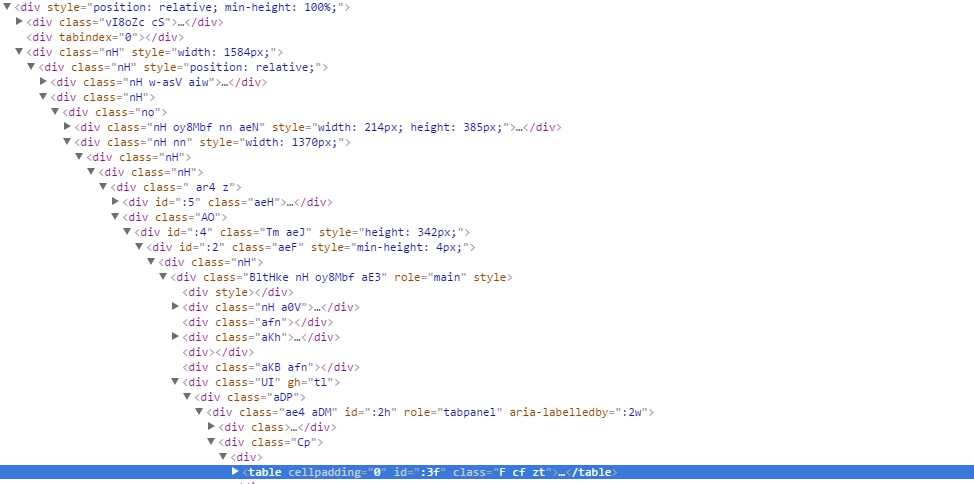
\includegraphics[width=14cm]{kapitel2/bilder/2-custom-elements-div-suppe}
 \caption{Screenshot des DOMs der Applikation Google Mail}
 \label{fig:cusel}
\end{figure}

Sie besteht aus vielen geschachtelten \texttt{\textless{}div\textgreater{}}-Elementen und macht folgende strukturelle Probleme deutlich: Die Semantik der Elemente fehlt vollständig und es ist nicht ersichtlich was es darstellt und welche Funkionen es hat, wodurch die Applikation nur sehr schwer wartbar ist.

Dieser Problematik widmen sich die Custom Elements. Sie bieten eine neue \ac{API}, welche es ermöglicht, eigene, semantisch aussagekräftige \ac{HTML}-Elemente mit Eigenschaften und Funktionen zu definieren. Wird das obige Beispiel nun also mit Hilfe von Custom Elements umgesetzt, so könnte das zugehörige \ac{DOM} wie in Listing \ref{beamwc} dargestellt aussehen \cite{citeulike:13844982}.

\lstinputlisting[language=HTML,label=beamwc,caption=Beispiel einer Applikation mit Web Components]{kapitel2/listings/2-1.html}

Die Spezifikation des \ac{W3C} ermöglicht nicht nur das Erstellen eigenständiger Elemente, sondern auch das Erstellen von Elementen, welche native Elemente erweitern. Somit können die \ac{API}s von nativen \ac{HTML}-Elementen um eigene Eigenschaften und Funktionen erweitert werden.


\subsection{Neue Elemente registrieren}\label{neue-elemente-registrieren}

Um nun ein eigenes Custom Element zu definieren, muss der Name des Custom Elements laut der \ac{W3C}-Spezifikation zwingend einen Bindestrich enthalten, wie beispielsweise in \texttt{my-element}. Somit ist gewährleistet, dass der Parser des Browsers die Custom Elements von den nativen Elementen unterscheiden kann \cite{citeulike:13845061}. Ein neues Element wird mittels JavaScript mit der Funktion \texttt{document.registerElement('my-element');} registriert. Zusätzlich zum Namen des Elements kann optional der Prototyp des Elements angegeben werden. Dieser ist jedoch standardmäßig ein \texttt{HTMLElement}, somit also erst wichtig, wenn es darum geht, vorhandene Elemente zu erweitern (siehe Abschnitt \ref{vorhandene-elemente-erweitern-type-extensions}). Durch das Registrieren des Elements wird es in die Registry des Browsers geschrieben, welche dazu verwendet wird, die Definitionen der \ac{HTML}-Elemente aufzulösen \cite{citeulike:13844982}. Ist ein Element noch nicht definiert und nicht beim Browser registriert, steht aber im Markup der Webseite, wird dies keinen Fehler verursachen, da dieses Element das Interface von \texttt{HTMLUnkownElement} benutzen muss \cite{citeulike:13851253}.

Nachdem das Element beim Browser registriert wurde, muss es zunächst mittels der Anweisung \texttt{document.createElement(tagName);} erzeugt werden, der \texttt{tagName} ist hierbei der Name des zuvor registrierten Elements. Danach kann es imperativ per JavaScript mittels \texttt{document.body.appendChild(myelement);} oder deklarativ direkt im \ac{HTML}-Dokument mittels \texttt{\textless{}my-element\textgreater{}\textless{}my-element\textgreater{}} verwendet werden.

\noindent \cite[S. 127-138]{citeulike:13844975}


\subsection{Vorhandene Elemente erweitern (Type Extensions)}\label{vorhandene-elemente-erweitern-type-extensions}

Statt neue Elemente zu erzeugen, können sowohl native \ac{HTML}-Elemente als auch bereits erstellte Custom Elements durch prototypische Vererbung um Funktionen und Eigenschaften erweitert werden, was auch als ``Type Extension'' bezeichnet wird. Zusätzlich zum Namen des erweiterten Elements wird nun der Prototyp sowie der Name des zu erweiternden Elements der \texttt{registerElement}-Funktion als Parameter übergeben. Soll also ein erweitertes \texttt{button}-Element registriert werden, muss dies wie in Listing \ref{reebe} gemacht werden.

\lstinputlisting[language=JavaScript,label=reebe,caption=Registrieren eines erweiterten Button-Elements]{kapitel2/listings/2-2.js}

Das registrierte, erweiterte Element kann nun mit dem Namen des zu erweiternden Elements als erstem Parameter und dem Namen des erweiterten Elements als zweitem Parameter erzeugt werden. Alternativ kann es auch mit Hilfe des Konstruktors erzeugt werden (siehe Listing \ref{eeebe}) \cite{citeulike:13752379}.

\lstinputlisting[language=HTML,label=eeebe,caption=Erzeugen eines erweiterten Button-Elements]{kapitel2/listings/2-3.js}

Um es nun im \ac{DOM} zu benutzen, muss der Name des erweiterten Elements via dem Attribut \texttt{is=\dq elementName\dq} des erweiternden Elements angegeben werden. So wird der erweiterte Button deklarativ mittels \texttt{\textless{}button\ is=\dq button-extended\dq\textgreater{}\textless{}/button\textgreater{}} in das Dokument eingebunden.


\subsection{Eigenschaften und Methoden definieren}\label{eigenschaften-und-methoden-definieren}

Anhand des obigen Beispiels wird deutlich, wie ein Custom Element eingesetzt werden kann, jedoch sind die internen JavaScript-Mechanismen nicht ersichtlich. Custom Elements entfalten ihr vollständiges Potential jedoch erst, wenn man für diese auch eigene Eigenschaften und Methoden definiert. Wie bei nativen \ac{HTML}-Elementen ist das auch bei Custom Elements auf analoge Weise möglich \cite[S. 127-138]{citeulike:13844975}. So kann einem Element eine Funktion zugewiesen werden, in dem diese dessen Prototyp mittels einem nicht reservierten Namen angegeben wird. Selbiges gilt für eine neue Eigenschaft. Die Eigenschaften können, nachdem sie im Prototyp definiert wurden, im \ac{HTML}-Markup deklarativ konfiguriert werden (siehe Listing \ref{eumduk}). Eigene Elemente mit einem spezifischen Eigenverhalten und Aussehen, wie beispielsweise ein neuer Video-Player, sind dadurch mit einem Tag statt mit einem Gerüst aus \texttt{\textless{}div\textgreater{}}-Tags oder Ähnlichem umsetzbar.

\lstinputlisting[language=HTML,label=eumduk,caption=Eigenschaften und Methoden definieren und konfigurieren]{kapitel2/listings/2-4.html}


\subsection{Custom Element Lifecycle-Callbacks}\label{custom-element-lifecycle-callbacks}

Custom Elements bieten eine standardisierte \ac{API} an speziellen Methoden, den ``Custom Element Lifecycle-Callbacks'', welche es ermöglichen Funktionen zu unterschiedlichen Zeitpunkten - vom Registrieren bis zum Löschen eines Custom Elements - auszuführen. Diese ermöglichen es, zu bestimmen, wann und wie ein bestimmter Code des Custom Elements ausgeführt werden soll.

\begin{description}
  \item[createdCallback] Wird ausgeführt, wenn eine Instanz des Custom Elements mittels \texttt{var\ mybutton\ =\ document.createElement('custom-element')} erzeugt wurde.
  \item[attachedCallback] Wird ausgeführt, wenn ein Custom Element dem \ac{DOM} mittels der Funktion \texttt{document.body.appendChild(mybutton)} angehängt wurde.
  \item[detachedCallback] Wird ausgeführt, wenn ein Custom Element aus dem \ac{DOM} mittels der Funktion \texttt{document.body.removeChild(mybutton)} entfernt wurde.
  \item[attributeChangedCallback] Wird ausgeführt, wenn ein Attribut eines Custom Elements mittels \texttt{MyElement.setAttribute()} geändert wurde.
\end{description}

So können die Lifecycle-Callbacks für ein neues erweitertes Button-Element, wie in Listing \ref{lccdebd} dargestellt, definiert werden \cite{citeulike:13844988}.

\lstinputlisting[language=HTML,label=lccdebd,caption=Lifecycle-Callbacks des erweiterten Buttons definieren]{kapitel2/listings/2-5.html}


\subsection{Styling von Custom Elements}\label{styling-von-custom-elements}

Das Styling von eigenen Custom Elements funktioniert analog dem Styling von nativen \ac{HTML}-Elementen indem der Name des Elements als \ac{CSS}-Selektor angegeben wird (siehe Listing \ref{seceudeb}). Erweiterte Elemente können mittels dem Attribut-Selektor in \ac{CSS} angesprochen werden \cite[S. 127-138]{citeulike:13844975}.


Ein Custom Element, welches zwar standardkonform deklariert oder erstellt, aber noch nicht beim Browser registriert wurde, ist ein ``Unresolved Element''. Steht dieses Element am Anfang des \ac{DOM}, wird jedoch erst später registriert, kann es nicht von \ac{CSS} angesprochen werden. Dadurch kann ein \ac{FOUC} entstehen, was bedeutet, dass das Element beim Laden der Seite nicht gestylt dargestellt wird, sondern das definierte Aussehen erst übernimmt, nachdem es registriert wurde. Um dies zu verhindern, sieht die \ac{HTML}-Spezifikation eine neue \ac{CSS}-Pseudoklasse \texttt{:unresolved} (siehe Listing \ref{seceudeb}) vor, welche deklarierte, aber nicht registrierte Elemente anspricht. Somit können diese Elemente initial beim Laden der Seite ausgeblendet und nach dem Registrieren wieder eingeblendet werden \cite{citeulike:13844984}.

\lstinputlisting[language=HTML,label=seceudeb,caption=Styling eines Custom Element und des erweiterten Button]{kapitel2/listings/2-6.css}

\subsection{Browserunterstützung}\label{custom-elements-browserunterstuetzung}

Custom Elements sind noch nicht vom \ac{W3C} standardisiert, sondern befinden sich noch im Status eines ``Working Draft'' \cite{citeulike:13845061}. Sie werden deshalb bisher nur von Google Chrome ab Version 43 und Opera ab Version 33 nativ unterstützt (siehe Abbildung \ref{fig:buce}) \cite{citeulike:13844983}.

\begin{figure}[htbp]
 \centering
 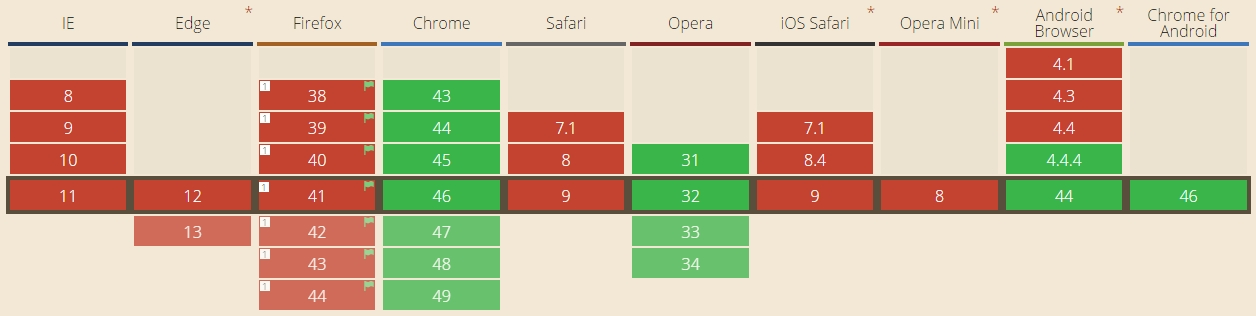
\includegraphics[width=\linewidth]{kapitel2/bilder/2-custom-elements-browserunterstuetzung}
 \caption{Browserunterstützung von Custom Elements}
 \label{fig:buce}
\end{figure}

\section{Shadow DOM}\label{shadow-dom}

Durch Kapselung ist es möglich, Details eines Objektes von anderen Teilen des Programms zu verstecken. Das Programm muss nur wissen, wie es auf die benötigten Funktionen zugreift, jedoch nicht, wie das Objekt die Funktionen intern umsetzt. Dieses Konzept ist in allen objektorientierten Programmiersprachen umgesetzt, jedoch nicht in der Webentwicklung. Beispielsweise kann das \ac{CSS} oder JavaScript, das für ein Element geschrieben ist, auch das \ac{CSS} oder JavaScript anderer Elemente beeinflussen. Je größer das Projekt wird, desto unübersichtlicher und komplexer wird es, zu gewährleisten, dass \ac{CSS} oder JavaScript sich nicht ungewollt auf andere Teile der Webseite auswirkt. Diesem Problem widmet sich das sogenannte Shadow \ac{DOM}, welches ein Sub-\ac{DOM} unterhalb eines Elements darstellt und es ermöglicht, \ac{HTML} und \ac{CSS} in sich zu kapseln und zu verstecken. Als Kontrast zu Bezeichnung ``Shadow \ac{DOM}'' wird das reguläre des Hauptdokuments auch oft als ``Light \ac{DOM}'' bezeichnet. Das Shadow \ac{DOM} wird bereits in \ac{HTML}5 standardmäßig eingesetzt, wie beispielsweise im \texttt{\textless{}video\textgreater{}}-Tag. Beim Inspizieren des Elements mit Hilfe der Chrome Developer Tools oder den Firefox-Entwicklungswerkzeugen wird deutlich, dass das \texttt{\textless{}video\textgreater{}}-Tag ein Shadow \ac{DOM} beinhaltet, welcher die Steuerelemente des Videos erzeugt. Neben dem \texttt{\textless{}video\textgreater{}}-Tag sind auch die verschiedenen \texttt{\textless{}input\textgreater{}}-Elemente, wie z.B. das \texttt{\textless{}input\ type=\dq password\dq \textgreater{}} (siehe Abbildung \ref{fig:itpelem}) mit einem Shadow \ac{DOM} ausgestattet \cite[S. 109-126]{citeulike:13844975}.

\begin{figure}[htbp]
 \centering
 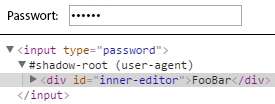
\includegraphics{kapitel2/bilder/3-shadow-dom-input-type-password}
 \caption{Passwort-Input-Element}
 \label{fig:itpelem}
\end{figure}


\subsection{Shadow DOM nach W3C}\label{shadow-dom-nach-w3c}

\begin{figure}[htbp]
 \centering
 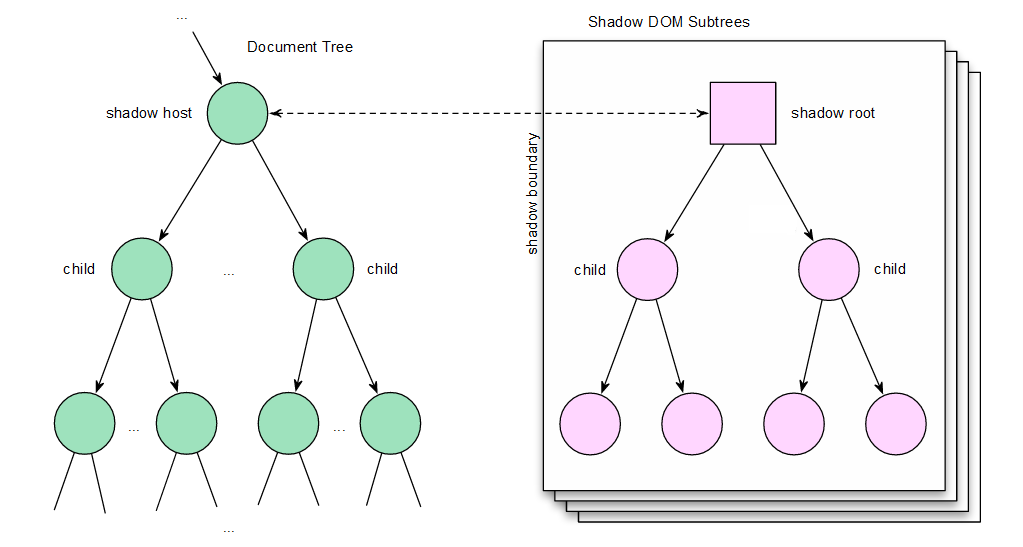
\includegraphics[width=\linewidth]{kapitel2/bilder/3-shadow-dom-shadow-boundary}
 \caption{Shadow \ac{DOM} und Shadow Boundary nach W3C}
 \label{fig:sdsbnw3c}
\end{figure}

Wie auf Abbildung \ref{fig:sdsbnw3c} zu sehen, liegt das Shadow \ac{DOM} dabei parallel zu dem \ac{DOM}-Knoten des beinhaltenden Elements. Ein Knoten im Document Tree (links abgebildet) wird als ``Shadow Host'' - ein Element, welches ein Shadow \ac{DOM} beinhaltet - markiert. Die gestrichelte Linie zeigt die Referenz zu der entsprechenden Shadow \ac{DOM} Wurzel, dem ``Shadow Root''. Die Referenz geht dabei durch die sogenannte ``Shadow Boundary'', welche es ermöglicht, den Shadow \ac{DOM}, und alles was dieser beinhaltet, zu kapseln \cite{citeulike:13851350}. Dies verhindert, dass externes \ac{CSS} oder JavaScript das interne Markup oder umgekehrt internes \ac{CSS} oder JavaScript den Light \ac{DOM} oder andere Shadow \ac{DOM}s ungewollt beeinflussen können. Ein Element kann auch mehrere Shadow \ac{DOM} Wurzeln referenzieren, allerdings wird nur die zuletzt hinzugefügte vom Browser gerendert, da dieser zum Rendern einen \ac{LIFO} Stack benutzt. Dabei wird der zuletzt hinzugefügte Shadow Tree ``Youngest Tree'' genannt, der jeweils zuvor hinzugefügte Shadow Tree wird ``Older Tree'' genannt. Das dynamische Hinzufügen von Shadow \ac{DOM}s ermöglicht es, die Inhalte der Webseite nach dem Rendern zu ändern.


\subsection{Content Projection}\label{content-projection}

Neben dem vom Shadow \ac{DOM} vorgegebenen \ac{HTML}, können auch Inhalte aus dem Light \ac{DOM} in den Shadow \ac{DOM} projiziert werden. Der Shadow \ac{DOM} nimmt dabei die zu projizierenden Inhalte und projiziert sie an der vorgegebenen Stelle im Shadow \ac{DOM}. Die Inhalte bleiben dabei an der ursprünglichen Stelle im \ac{DOM} stehen und werden nicht verschoben, gelöscht oder geändert. Der Shadow \ac{DOM} ermöglicht es somit eigenes, gekapseltes \ac{HTML} sowie dynamische Inhalte des Light \ac{DOM} anzuzeigen. Diese Projektion der Inhalte aus dem Light \ac{DOM} in den Shadow \ac{DOM} erfolgt mittels sogenannten ``Insertion Points''. Diese sind vom Entwickler definierte Stellen im Shadow \ac{DOM}, in welche der Inhalt projiziert wird. Es kann hierbei zwischen 2 Arten von Insertion Points unterschieden werden.

\subsection{Insertion Points}\label{insertion-points}

Um das zu präsentierende \ac{HTML} und den Inhalt zu trennen, wird ein \texttt{\textless{}template\textgreater{}}-Tag benutzt. Dieses beinhaltet das komplette Markup, das im Shadow \ac{DOM} stehen und nicht nach außen sichtbar sein oder von \ac{CSS} oder JavaScript von außen manipuliert werden soll. Um nun Inhalte aus dem Light \ac{DOM} in das \ac{DOM} des \texttt{\textless{}template\textgreater{}}-Tags zu projizieren, muss das \texttt{\textless{}template\textgreater{}}-Tag einen \texttt{\textless{}content\textgreater{}}-Tag beinhalten, in welchem die Inhalte von außen dargestellt werden sollen. Mittels \texttt{createShadowRoot()} wird das ausgewählte Element zu einem Shadow Host, also dem Shadow \ac{DOM} beinhaltendem Element gemacht. Der Inhalt des Templates wird geklont und dem Shadow Host angehängt. Das Shadow \ac{DOM} projiziert nun alle Inhalte des Shadow Roots in den \texttt{\textless{}content\textgreater{}}-Tag (siehe Listing \ref{tdueesd}) \cite{citeulike:13851404}.

\lstinputlisting[language=HTML,label=tdueesd,caption=Template-Definition und Erstellen eines Shadow \ac{DOM}s]{kapitel2/listings/3-1.html}

Im Light \ac{DOM} gerendert wird dabei nur der Text ``Inhalt'' des \texttt{\textless{}div\textgreater{}}-Tags mit der ID \texttt{shadow}, der Wrapper um das \texttt{\textless{}content\textgreater{}}-Tag wird nicht gerendert, da dieser im Shadow \ac{DOM} steht. Somit wurde eine Trennung des präsentierenden \ac{HTML} und dem Inhalt erreicht, die Präsentation erfolgt im Shadow \ac{DOM}, der Inhalt steht im Light \ac{DOM}. Werden nun mehrere \ac{HTML}-Elemente oder Knoten in den Shadow \ac{DOM} projiziert, werden diese ``Distributed Nodes'' genannt. Diese Distributed Nodes sind nicht wirklich im Shadow \ac{DOM}, sondern werden nur in diesem gerendert, was bedeutet, dass sie auch von außen gestylt werden können, mehr dazu im Abschnitt \ref{styling-mit-css}. Des Weiteren können auch nur bestimmte Elemente in das Shadow \ac{DOM} projiziert werden, ermöglicht wird dies mit dem Attribut \texttt{select=\dq selector\dq} des \texttt{\textless{}content\textgreater{}}-Tags. Dabei können sowohl Namen von Elementen, als auch \ac{CSS} Selektoren verwendet werden \cite{citeulike:13851402}. Der Inhalt des \texttt{\textless{}content\textgreater{}}-Tags kann mit JavaScript nicht traversiert werden, beispielsweise gibt \texttt{console.log(shadow.querySelector('content'));} \texttt{null} aus. Allerdings ist es erlaubt, die Distributed Nodes mittels \texttt{.getDistributedNodes()} auszugeben. Dies lässt darauf schließen, dass der Shadow \ac{DOM} nicht als Sicherheits-Feature angedacht ist, da die Inhalte nicht komplett isoliert sind.

\subsection{Shadow Insertion Points}\label{shadow-insertion-points}

Neben den \texttt{\textless{}content\textgreater{}}-Tags gibt es auch die \texttt{\textless{}shadow\textgreater{}}-Tags, welche Shadow Insertion Points genannt werden. Shadow Insertion Points sind ebenso wie Insertion Points Platzhalter, doch statt einem Platzhalter für den Inhalt eines Hosts, sind sie Platzhalter für Shadow \ac{DOM}s. Falls jedoch mehrere Shadow Insertion Points in einem Shadow \ac{DOM} sind, wird nur der erste berücksichtigt, die restlichen werden ignoriert. Wenn nun mehrere Shadow \ac{DOM}s projiziert werden sollen, muss im zuletzt hinzugefügten Shadow \ac{DOM} - dem sogenannten ``Younger Tree'' - ein \texttt{\textless{}shadow\textgreater{}}-Tag stehen, dieser rendert den zuvor hinzugefügten Shadow \ac{DOM} - den sogenannten ``Older Tree''. Somit wird eine Schachtelung mehrerer Shadow \ac{DOM}s ermöglicht \cite{citeulike:13851421}.

\subsection{Styling mit CSS}\label{styling-mit-css}

Eines der Hauptfeatures des Shadow \ac{DOM}s ist die Shadow Boundary, welche Kapselung von Stylesheets standardmäßig mit sich bringt. Sie gewährleistet, dass Style-Regeln des Light \ac{DOM} nicht den Shadow \ac{DOM} beeinflussen und umgekehrt \cite{citeulike:13851334}. Dies gilt jedoch nur für die Präsentation des Inhalts, nicht für den Inhalt selbst. Nachfolgend wird auf die wichtigsten Selektoren für das Styling eingegangen.

\begin{description}
  \item[:host] Das Host-Element des Shadow \ac{DOM}s kann mittels dem Pseudoselektor \texttt{:host} angesprochen werden. Dabei kann dem Selektor optional auch ein Selektor mit übergeben werden wie beispielsweise mit \texttt{:host(.myHostElement)}. Mit diesem Selektor ist es möglich, nur Hosts, welche diese Klasse haben, anzusprechen. Zu beachten ist, dass das Host-Element von außen gestylt werden kann, also die Regeln des \texttt{:host}-Selektors überschreiben kann. Des Weiteren funktioniert der \texttt{:host}-Selektor nur im Kontext eines Shadow \ac{DOM}s, man kann ihn also nicht außerhalb benutzen. Besonders wichtig ist dieser Selektor, wenn auf die Aktivität der Benutzer reagiert werden muss. So kann innerhalb des Shadow \ac{DOM}s angegeben werden, wie das Host Element beispielsweise beim Hover mit der Maus auszusehen hat.
  \item[:host-context()] Je nach Kontext eines Elements kann es vorkommen, dass Elemente unterschiedlich dargestellt werden müssen. Das wohl am häufigsten auftretende Beispiel hierfür ist das Theming. Themes ermöglichen es, Webseiteninhalte auf unterschiedliche Arten darzustellen. Oftmals bietet eine Webseite oder eine Applikation mehrere Themes für die Benutzer an, zwischen welchen sie wechseln können. Mit dem \texttt{:host-context()}-Selektor wird es möglich, ein Host-Element je nach Klasse des übergeordneten Elements - dem Parent-Element - zu definieren. Hat ein Host-Element mehrere Style-Definitionen, so werden diese nach der Klasse des Parent-Elements getriggert. Soll eine Style-Definition beispielsweise nur angewendet werden, wenn das umschließende Element die Klasse \texttt{theme-1} hat, so kann das mit \texttt{:host-context(.theme-1)} erreicht werden.
\end{description}


\subsection{Styling des Shadow DOM von außerhalb}\label{styling-des-shadow-dom-von-ausserhalb}

Trotz der Kapselung von Shadow \ac{DOM}s ist es mit speziellen Selektoren möglich, die Shadow Boundary zu durchbrechen. So können Style-Regeln für Shadow Hosts oder in ihm enthaltene Elemente vom Elterndokument definiert werden \cite{citeulike:13883067}.

\begin{description}
  \item[::shadow] Falls ein Element nun einen Shadow Tree beinhalten sollte, so kann dieses mit der entsprechenden Klasse oder ID sowie dem \texttt{::shadow}-Selektor angesprochen werden. Jedoch können mit diesem Selektor keine allgemeingültigen Regeln erstellt werden. Stattdessen muss stets ein in dem Shadow Tree enthaltener Elementname angesprochen werden. Nimmt man sich nun die Content Insertion Points zur Hilfe, so ist es dennoch möglich, Regeln für mehrere unterschiedliche Elemente zu definieren. Die Selektor-Kombination \texttt{\#my-element::shadow\ content} Spricht nun alle \texttt{\textless{}content\textgreater{}}-Tags an, welche im Shadow Tree des Elements \texttt{\#my-element} vorhanden sind. Da in diesen \texttt{\textless{}content\textgreater{}}-Tag wiederum die Inhalte hineinprojiziert werden, werden die Regeln für die projizierten Elemente angewendet. Sollten nun noch weitere Shadow \ac{DOM}s in diesem Element geschachtelt sein, so werden die Regeln jedoch nicht für diese angewandt, sondern nur für das direkt folgende Kind des Elements \texttt{\#my-element}.
  \item[\textgreater{}\textgreater{}\textgreater{}] Dieser Kombinator ist ähnlich dem \texttt{::shadow}-Selektor. Er bricht jedoch durch sämtliche Shadow Boundaries und wendet die Regeln auf alle gefundenen Elemente an. Dies gilt - im Gegensatz zum \texttt{::shadow}-Selektor - auch für geschachtelte Shadow Trees. Mit dem Selektor \texttt{my-element\ \textgreater{}\textgreater{}\textgreater{}\ span} werden also alle im Element \texttt{\textless{}my-element\textgreater{}} sowie in dessen geschachtelten Shadow Trees enthaltenen \texttt{\textless{}span\textgreater{}}-Elemente angesprochen.
  \item[::slotted] Die Kombination \texttt{\#my-element::shadow\ content} zeigt die Möglichkeit, wie die Inhalte eine Shadow \ac{DOM}s von außen gestylt werden können. Sollen jene in den Content Insertion Points enthaltenen ELemente jedoch von innerhalb gestylt werden, so ist dies mit dem \texttt{::slotted}-Selektor möglich. Ist innerhalb eines Elements die Regel \texttt{::slotted\ p} definiert, so werden alle in den Shadow \ac{DOM} projizierten \texttt{\textless{}p\textgreater{}}-Tags angesprochen.
\end{description}


\subsection{CSS-Variablen}\label{css-variablen}

Die oben gezeigten Selektoren und Kombinatoren eignen sich hervorragend um die Shadow Boundary zu durchdringen und eigene Styles den Elementen aufzuzwingen. Jedoch sprengen sie das Prinzip der Kapselung, das man mit Web Components zu gewinnen versucht. Dennoch haben sie ihre Existenzberechtigung. Sie ermöglichen es den Entwicklern, fremde Components sowie native \ac{HTML}-Elemente, die einen Shadow \ac{DOM} benutzen, wie z.B. \texttt{\textless{}video\textgreater{}} oder \texttt{\textless{}input\textgreater{}}-Elemente, zu stylen. Allerdings sollte bei ihrer Anwendung äußerst vorsichtig gearbeitet werden, besonders da sie schnell missbraucht werden können.

Ein Ansatz zur Lösung dieser Problematik sind \ac{CSS}-Variablen. Mit ihnen können Elemente in ihrem Shadow \ac{DOM} Variablen für die inneren Styles bereit halten, welche von außerhalb des Shadow \ac{DOM}s instanziiert werden können. Dadurch ist es möglich, das innere Styling eines Elements nach außen zu reichen. Statt die Barriere nun zu durchbrechen, können Elemente miteinander kommunizieren. Es wird somit eine Style-Schnittstelle geschaffen \cite{citeulike:13883381}. Ein Element \texttt{my-element} kann nun in dessen Shadow \ac{DOM} beispielsweise die Schriftfarbe mit \texttt{color} definieren. Doch statt einem Wert wird nun der Name der nach außen sichtbaren Variablen angegeben. Die Syntax hierfür lautet \texttt{var(-\/-varable-name,\ red)}, wobei \texttt{red} hier der Standardwert ist, falls die Variable `--variable-name` von außen nicht gesetzt wird. Nachdem die Variable definiert wurde, kann sie von außerhalb des Shadow \ac{DOM} mittels der Regel \texttt{\#my-shadow-host\ \{\ -\/-varable-name:\ blue;\ \}} überschrieben werden.

\subsection{Beispiel eines Shadow DOMs mit Template und CSS}\label{beispiel-eines-shadow-doms-mit-template-und-css}

Listing \ref{biesdmtucss} zeigt eine exemplarische Implementierung eines Shadow \ac{DOM}s, welcher gekapseltes \ac{CSS} und JavaScript beinhaltet.

\lstinputlisting[language=HTML,label=biesdmtucss,caption=Beispielimplementierung eines Shadow \ac{DOM}s mit Template und \ac{CSS}]{kapitel2/listings/3-2.html}

Das obige Beispiel wird vom Browser, wie in Abbildung \ref{fig:shadowdombeispiel} dargestellt, gerendert.

\begin{figure}[htbp]
 \centering
 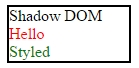
\includegraphics{kapitel2/bilder/3-shadow-dom-beispiel}
 \caption{Shadow DOM Beispiel}
 \label{fig:shadowdombeispiel}
\end{figure}

Anhand des gerenderten Outputs werden einige Dinge deutlich. Mit der Angabe des \texttt{select}-Attributs, werden im \texttt{\textless{}content\textgreater{}}-Tag nur die \texttt{\textless{}div\textgreater{}}-Tags mit der ID \texttt{hello} aus dem Shadow Root, welcher per \texttt{var\ root\ =\ document.querySelector('\#hello').createShadowRoot()} erzeugt wird, gerendert. Der Paragraph mit der ID \texttt{hidden} wird hingegen nicht gerendert, da er nicht im \texttt{select} mit inbegriffen ist. Die \ac{CSS}-Regel \texttt{.content\ \{\ background-color:\ khaki;\ \}} des Eltern-\ac{HTML}-Dokuments greift nicht, da die Styles des Shadow Roots durch die Shadow Boundary gekapselt werden. Die \ac{CSS} Regel \texttt{.styled\ \{\ color:\ green;\ \}} greift allerdings, da das \texttt{\textless{}div\textgreater{}}-Element mit der Klasse \texttt{styled} aus dem Light \ac{DOM} in den Shadow \ac{DOM} projiziert wird. Außerdem können innerhalb des Templates CSS-Regeln für die beinhaltenden Elemente definiert werden, somit wird das \texttt{\textless{}div\textgreater{}}-Element ohne eine zugehörige Klasse mit der Regel \texttt{.content\ \{\ color:\ red;\ \}} auch dementsprechend in Rot gerendert.


\subsection{Browserunterstützung}\label{shadow-dom-browserunterstuetzung}

Der Shadow \ac{DOM} ist noch nicht vom \ac{W3C} standardisiert, sondern befindet sich noch im Status eines ``Working Draft'' \cite{citeulike:13879687}. Er wird deshalb bisher nur von Google Chrome ab Version 43 und Opera ab Version 33 nativ unterstützt (siehe Abbildung \ref{fig:shadowdombrowser}) \cite{citeulike:13883407}.

\begin{figure}[htbp]
 \centering
 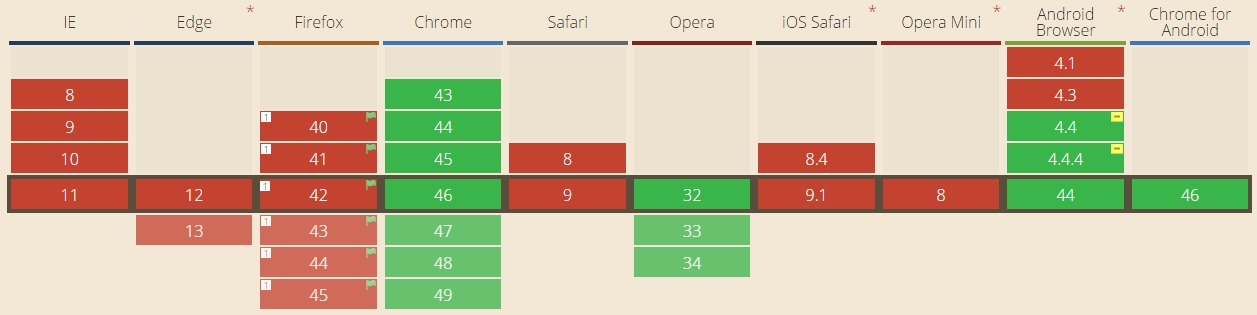
\includegraphics[width=\linewidth]{kapitel2/bilder/3-shadow-dom-browserunterstuetzung}
 \caption{Browserunterstützung des Shadow DOMs}
 \label{fig:shadowdombrowser}
\end{figure}

\section{HTML Templates}\label{html-templates}

\todo{Buchquelle hinzufügen [S.101-107]}

Bisher gibt es ohne eine Library oder Framework keine Möglichkeit, im Browser Templates zu rendern, um bestimmte Inhalte der Seite zur Laufzeit auszuwechseln. Die Technologie ``\ac{HTML} Templates'' ist eine neue Technologie im Rahmen der Web Components und versucht eben dieses Problem mit einer nativen \ac{API} zu lösen.

Im Kontext der Entwicklung einer \ac{MVC}-Applikation ist der Mechanismus der Darstellung der Präsentations-Schicht, auch View genannt, besonders wichtig. Bisher ist dies ohne weiteres problemlos serverseitig in PHP, Ruby oder ähnlichem möglich, da diese Sprachen für die Webentwicklung eine Syntax für die Einbettung dynamischer Inhalte in \ac{HTML} bieten, die sogenannten Templates. Im Gegensatz zu den serverseitigen Technologien, existieren Client-seitige Lösungen bisher nur als Library oder Framework, wie beispielsweise Mustache.js oder Handlebars.js \cite{citeulike:13853015}. Eine native Möglichkeit, Templates auf der Client-Seite zu benutzen, fehlt bisher hingegen. An diese Problematik setzen die \ac{HTML} Templates an, durch welche diese Technik auch Einzug in den Browser erhält.

\begin{quote}
Das \ac{HTML} template-Element \textless{}template\textgreater{} dient dazu, Client-seitige Inhalte zu gruppieren, die nicht gerendert werden, wenn die Seite geladen wird, sondern anschließend zur Laufzeit mittels JavaScript gerendert werden können. Template kann als Inhaltsfragment aufgefasst werden, das für eine spätere Verwendung im Dokument gespeichert wird. \cite{citeulike:13852997}
\end{quote}


\subsection{Bisherige Umsetzung von Templates im Browser}\label{bisherige-umsetzung-von-templates-im-browser}

Dennoch gibt es diverse Methoden, diese Technologie im Browser zu simulieren. Diese sind jedoch eher als Hacks zu betrachten, da ihre eingesetzten Mittel nicht für dieses Problem gedacht sind. Sie bringen also einige Nachteile mit sich. Einige dieser Methoden werden nachfolgend aufgezeigt \cite{citeulike:13853018}.\\

\textbf{Via verstecktem \texttt{\textless{}div\textgreater{}}-Element}

Das Listing \ref{uetmedb} zeigt die Umsetzung eines Templates mit Hilfe eines \texttt{\textless{}div\textgreater{}}-Blocks, der via \ac{CSS} versteckt wird.

\lstinputlisting[language=HTML,label=uetmedb,caption=Umsetzung eines Templates mit einem \texttt{\textless{}div\textgreater{}}-Block]{kapitel2/listings/4-1.html}

Der entscheidende Nachteil dieser Methode ist, dass alle Ressourcen, also alle verlinkten Dateien, beim Laden der Webseite auch heruntergeladen werden. Zwar werden sie nicht angezeigt, dennoch verursachen sie eine große Datenmenge, welche initial übertragen werden muss. Dies geschieht in diesem Fall selbst wenn die Ressourcen eventuell erst später oder gar nicht benötigt werden, was eine massive Einschränkung der verfügbaren Bandbreite und Browser-Performance mit sich bringen kann. Des Weiteren kann es sich als schwierig erweisen, ein solches Code-Fragment zu stylen oder gar Themes auf mehrere solcher Fragmente anzuwenden. Eine Webseite, die das Template verwendet, muss alle \ac{CSS}-Regeln für das Template mit \texttt{\#mydivtemplate} erstellen, welche sich unter Umständen auf andere Teile der Webseite auswirken können. Eine Kapselung wird hier somit nicht vorgesehen.\\

\textbf{Via \texttt{\textless{}script\textgreater{}}-Element:}

Eine weitere Möglichkeit ein Template umzusetzen besteht darin, den Inhalt eines Templates in ein \texttt{\textless{}script\textgreater{}}-Tag zu schreiben, wie in Listing \ref{uetmese} gezeigt.

\lstinputlisting[language=HTML,label=uetmese,caption=Umsetzung eines Templates mit einem \texttt{\textless{}script\textgreater{}}-Element]{kapitel2/listings/4-2.html}

Wie bei dem Beispiel mit einem \texttt{\textless{}div\textgreater{}}-Element wird auch bei dieser Methode der Inhalt nicht gerendert, da ein \texttt{\textless{}script\textgreater{}}-Tag standardmäßig die \ac{CSS}-Eigenschaft \texttt{display:\ none} hat. In diesem Fall werden jedoch die benötigten Ressourcen nicht geladen, somit gibt es keine zusätzlichen Performance-Einbrüche. Es besteht dennoch ein Nachteil, auf den besonders geachtet werden muss: Der Inhalt des \texttt{\textless{}script\textgreater{}}-Tags muss via \texttt{innerHTML} in den \ac{DOM} geklont werden, was eine mögliche \ac{XSS} Sicherheitslücke darstellen kann. Es muss also abgewägt werden, welche der Nachteile für den Entwickler am ehesten hinnehmbar sind und welche Methode verwendet werden soll.


\subsection{Das \texorpdfstring{\texttt{\textless{}template\textgreater{}}-Tag}{\textless{}template\textgreater{}-Tag}}\label{template-tag}

Den Problemen der oben genannten Methoden widmet sich der \texttt{\textless{}template\textgreater{}}-Tag, welcher eine native und sichere Methode für das Einbinden von dynamischen Inhalten etabliert. Das Template und die darin enthaltenen Inhalte werden beim Rendern des Webseite vollständig ignoriert, sie werden weder angezeigt, noch werden ihre benötigten Inhalte beim Laden der Webseite mitgeladen. Ebenso werden enthaltene JavaScripts nicht ausgeführt, auch kann JavaScript von außen nicht in das Template hinein traversieren. In Listing \ref{gsetmcssujs} wird die grobe Struktur eines einfachen Templates, das mit Hilfe des \texttt{\textless{}template\textgreater{}}-Tags umgesetzt wird, dargestellt.

\lstinputlisting[language=HTML,label=gsetmcssujs,caption=Grobe Struktur eines Templates mit \ac{CSS} und JavaScript]{kapitel2/listings/4-2.html}


\subsection{Benutzung}\label{benutzung}

Natürlich soll ein Template nicht nur im Quelltext stehen, damit es existiert, sondern es soll dynamisch zur Laufzeit geladen und gerendert werden. Dabei kann es an einer beliebigen Stelle im Quelltext stehen. Um es aus dem Quelltext in den \ac{DOM} zu importieren und zu rendern, muss es zunächst via JavaScript selektiert werden, was mit der Funktion \texttt{var\ template\ =\ document.querySelector('\#mytemplate');} möglich ist. Mit der Funktion \texttt{var\ templateClone\ =\ document.importNode(template.content,\ true);} wird eine Kopie als \ac{DOM}-Knoten des Templates erstellt. Als erster Parameter wird dabei der Inhalt des Templates (\texttt{template.content}) und als zweiter Parameter ein Boolean für \texttt{deep}, welcher angibt ob auch Kinderknoten geklont werden sollen. Nun kann der Inhalt des Templates mittels \texttt{document.body.appendChild(templateClone);} an einer beliebigen Stelle des \ac{DOM} eingefügt werden.


\subsection{Vorteile}\label{vorteile}

Die Vorteile dieser nativen Implementierung für Templates sind vielfältig. So sind \ac{HTML} Templates ein fertiges Gerüst an \ac{HTML}, das nicht nachträglich mit JavaScript modifiziert werden muss, es kann aus dem Quelltext kopiert und beliebig oft und an beliebiger Stelle in den \ac{DOM} der Webseite eingefügt werden. Erst beim einfügen in den \ac{DOM} werden die Inhalte tatsächlich gerendert und Abhängigkeiten nachgeladen. Darunter fallen auch enthaltene Styles oder JavaScript-Codes, welche erst beim Einfügen angewendet und ausgeführt werden. So werden auch externe Stylesheets, JavaScript-Dateien oder Bilder und Videos erst dann geladen und abgespielt, wenn sie tatsächlich benötigt werden. Dadurch können auch beliebig viele \texttt{\textless{}template\textgreater{}}-Tags ohne signifikanten Performance-Einbruch im Quelltext stehen, da nur ihr Markup übertragen wird, es jedoch nicht vom Browser geparst werden muss. Des Weiteren sind Templates komplett vor dem \ac{DOM} versteckt, will man beispielsweise mit JavaScript in das Template mittels \texttt{document.getElementById('\#mytemplate\ .text')} hinein traversieren, so gibt die Funktion `null` zurück. Der abschließende und wohl auch größte Vorteil ist, dass mit JavaScript auf das Template zugegriffen werden und es an anderer Stelle dynamisch eingebunden werden kann.
Falls nun jedoch in einem Template mehrere weitere Templates geschachtelt sind, so muss jedes dieser Templates einzeln aus dem aktiven Template im \ac{DOM} kopiert und wieder eingefügt werden um es zu aktivieren.


\subsection{Browserunterstützung}\label{html-templates-browserunterstuetzung}

\ac{HTML} Templates sind zum Stand dieser Arbeit als einzige Technologie des Web Components Technology Stacks vom \ac{W3C} als Standard erklärt worden \cite{citeulike:13853159}. Somit ist auch die Browserunterstützung in den aktuellen Browsern, bis auf den Internet Explorer, sehr gut (siehe Abbildung \ref{fig:bdhtmltt}). Sie sind des Weiteren die einzige Technologie der Web Components, die bisher von Microsofts Edge ab Version 13 unterstützt werden.

\begin{figure}[htbp]
 \centering
 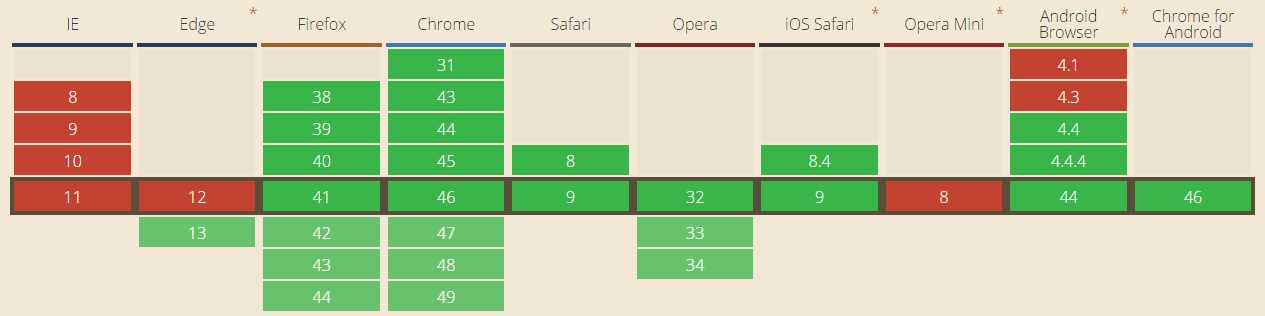
\includegraphics[width=\linewidth]{kapitel2/bilder/4-html-templates-browserunterstuetzung}
 \caption{Browserunterstützung des HTML Template Tags}
 \label{fig:bdhtmltt}
\end{figure}

\section{HTML Imports}\label{html-imports}

Bisher erlauben es praktisch alle Plattformen, Codeteile zu importieren und zu verwenden, nur nicht das Web bzw. \ac{HTML}. Das heutige \ac{HTML} ermöglicht es externe Stylesheets, JavaScript Dateien, Bilder etc. in ein \ac{HTML} Dokument zu importieren, \ac{HTML}-Dateien selbst können jedoch nicht importiert werden. Auch ist es nicht möglich, alle benötigten Dateien in einer Ressource zu bündeln und als einzige Abhängigkeit zu importieren. \ac{HTML} Imports versuchen eben dieses Problem zu lösen. So soll es möglich sein, \ac{HTML}-Dateien und wiederum \ac{HTML}-Dateien in \ac{HTML}-Dateien zu importieren. So können auch verschiedene benötigte Dateien in einer \ac{HTML}-Datei gesammelt und mit nur einem Import in die Seite eingebunden werden. Doppelte Abhängigkeiten sollen dadurch automatisch aufgelöst werden, sodass Dateien, die mehrmals eingebunden werden sollten, automatisch effektiv nur einmal heruntergeladen werden.


\subsection{HTML-Dateien importieren}\label{html-dateien-importieren}

Imports von \ac{HTML}-Dateien werden, wie andere Imports auch, per \texttt{\textless{}link\textgreater{}}-Tag deklariert. Neu ist jedoch der Wert des \texttt{rel}-Attributes, welches auf \texttt{import} gesetzt wird \cite[S. 139-147]{citeulike:13844975}. So kann beispielsweise das Bootstrap-Frame\-work statt wie bisher mit mehreren Imports mit nur einem Import eingebunden werden. Bisher könnte die Einbindung unter Berücksichtigung der Abhängigkeiten wie in Listing \ref{evbohtmli} aussehen.

\lstinputlisting[language=HTML,label=evbohtmli,caption=Einbindung von Bootstrap ohne \ac{HTML} Imports]{kapitel2/listings/5-1.html}

Stattdessen kann dieses Markup nun in ein einziges \ac{HTML} Dokument, welches alle Abhängigkeiten verwaltet, geschrieben werden. Dieses wird dann mit einem einzigen Import \texttt{\textless{}link\ rel=\dq import\dq\ href=\dq bootstrap.html\dq\textgreater{}} in das eigene \ac{HTML} Dokument importiert.

Es ist jedoch zu beachten, dass \ac{HTML} Imports nur auf Ressourcen der gleichen Quelle, also dem gleichen Host, respektive der gleichen Domain zugreifen können. Imports von \ac{HTML}-Dateien von verschiedenen Quellen stellen eine Sicherheitslücke dar, da Webbrowser die \ac{SOP} verfolgen.

\begin{quote}
The same-origin policy restricts how a document or script loaded from one origin can interact with a resource from another origin. It is a critical security mechanism for isolating potentially malicious documents. \cite{citeulike:13853253}
\end{quote}

Sollte das jedoch dennoch erlaubt werden, so muss das \ac{CORS} für die entsprechende Domain auf dem Server aktiviert werden.

\begin{quote}
These restrictions prevent a client-side Web application running from one origin from obtaining data retrieved from another origin, and also limit unsafe \ac{HTTP} requests that can be automatically launched toward destinations that differ from the running application's origin. \cite{citeulike:13853643}
\end{quote}


\subsection{Auf importierte Inhalte zugreifen}\label{html-imports-verwenden}

Importierte \ac{HTML}-Dateien werden nicht nur in das Dokument eingefügt, sondern vom Parser verarbeitet, das bedeutet, dass mit JavaScript auf das \ac{DOM} des Imports zugegriffen werden kann. Wenn sie vom Parser verarbeitet worden sind, sind sie zwar verfügbar, allerdings werden die Inhalte nicht angezeigt bis sie mittels JavaScript in das \ac{DOM} eingefügt werden. Ihre enthaltenen Scripte werden also ausgeführt, Styles und \ac{HTML}-Knoten werden jedoch ignoriert. Um nun die Inhalte eines Imports auf der Seite einzubinden, muss auf die \texttt{.import} Eigenschaft des \texttt{\textless{}link\textgreater{}}-Tags mit dem Import zugegriffen werden \texttt{var\ content\ =\ document.querySelector('link{[}rel=\dq import\dq{]}').import;}. Nun kann auf das \ac{DOM} des Imports zugegriffen werden. So kann ein enthaltenes Element mit der Klasse \texttt{element} mit \texttt{var\ el\ =\ content.querySelector('.element');} geklont und anschließend durch \texttt{document.body.appendChild(el.cloneNode(true));} in das eigene \ac{DOM} eingefügt werden. Falls es jedoch mehrere Imports geben sollte, können den Imports IDs zugewiesen werden, anhand derer die Imports voneinander unterschieden werden können (siehe Listing \ref{euvvhtmli}) \cite{citeulike:13853724}.

\lstinputlisting[language=HTML,label=euvvhtmli,caption=Einbinden und Verwenden von \ac{HTML} Imports]{kapitel2/listings/5-2.html}


\subsection{Abhängigkeiten verwalten}\label{abhuxe4ngigkeiten-verwalten}

Jedoch kann es vorkommen, dass mehrere eingebundenen Bibliotheken die gleichen Abhängigkeiten haben und diese verwaltet werden müssen. Sollte dies nicht sorgfältig gemacht werden, können unerwartete Fehler auftreten, die mitunter nur schwer zu lokalisieren sind. \ac{HTML} Imports verwalten Abhängigkeiten automatisch. Um das zu erreichen, werden die Abhängigkeiten gebündelt und in eine zu importierende \ac{HTML}-Datei geschrieben. Haben mehrere Imports die gleichen Abhängigkeiten (siehe Listing \ref{ahvmhtmli}), werden diese vom Browser erkannt und nur einmal heruntergeladen. Mehrfachdownloads und Konflikte der Abhängigkeiten werden so verhindert \cite{citeulike:13853700}.

\lstinputlisting[language=HTML,label=ahvmhtmli,caption=Abhängigkeitsverwaltung mit \ac{HTML} Imports]{kapitel2/listings/5-3.html}

Selbst wenn die jQuery-Library in mehreren Dateien eingebunden wird, wird hier sie dennoch nur einmal übertragen. Wenn nun fremde \ac{HTML}-Dateien eingebunden werden, muss auch nicht auf die Reihenfolge der Imports geachtet werden, da diese selbst ihre Abhängigkeiten beinhalten.


\subsection{Sub-Imports}\label{sub-imports}

Das obige Beispiel zeigt, dass \ac{HTML} Imports selbst wiederum auch \ac{HTML} Imports beinhalten können. Diese Imports werden Sub-Imports genannt und ermöglichen einen einfachen Austausch oder eine Erweiterungen von Abhängigkeiten innerhalb einer Komponente. Wenn eine Komponente A eine Abhängigkeit von einer Komponenten B hat und eine neue Version von Komponente B verfügbar ist, kann dies einfach in dem Import des Sub-Imports angepasst werden ohne den Import in der Eltern-\ac{HTML}-Datei anpassen zu müssen \cite{citeulike:13853647}.


\subsection{Performance}\label{html-import-performance}

Ein signifikantes Problem der \ac{HTML} Imports ist die Performance, welche bei komplexen Anwendungen schnell abfallen kann. Werden auf einer Seite mehrere Imports eingebunden, die selbst wiederum Imports beinhalten können, so steigt die Anzahl an Requests an den Server schnell exponentiell an, was die Webseite stark verlangsamen kann. Auch das Vorkommen von doppelten Abhängigkeiten kann die Anzahl an Requests in die Höhe treiben, doch da Browser die Abhängigkeiten nativ schon selbst de-duplizieren, kann dieses Problem in diesem Zusammenhang ignoriert werden \cite{citeulike:13853714}.

Dennoch sind viele Einzel-Requests ein gewünschtes Verhalten von Web Components, da sie bereits mit Blick auf Version 2 des \ac{HTTP}-Protokolls entwickelt wurden. In diesem können mehrere Requests in einer \ac{TCP}-Verbindung übertragen werden. Des Weiteren kann der Client die Priorität der angeforderten Dateien bestimmen, um Dateien mit einer hohen Priorität vor Dateien mit niedrigerer Priorität zu erhalten. Ebenso wird mit einer neuen Header-Kompression die zu übertragende Datenmenge verkleinert. Neu sind außerdem die sogenannten ``Server Pushes'', welche es dem Server ermöglichen, Nachrichten an den Client zu schicken, ohne dass dieser sie anfordern muss.

Voraussetzung hierfür ist jedoch die Unterstützung des neuen Protokolls seitens des Browsers. Bis auf den Internet Explorer und Safari unterstützen jedoch alle Browser \ac{HTTP}/2 schon ab frühen Versionen, allerdings nur bei mittels \ac{TLS} verschlüsselten Webseiten \cite{citeulike:13879562}. Der Anteil der über \ac{HTTP}/2 ausgelieferten Webseiten liegt momentan bei circa 3\% \cite{citeulike:13879575}.


\subsection{Asynchrones Laden von Imports}\label{asynchrones-laden-von-imports}

Das Rendern der Seite kann unter Umständen sehr lange dauern, da das in den Imports enthaltene JavaScript das Rendern blockiert. Um das zu verhindern und alle Dateien möglichst schnell laden zu können, ist ein \texttt{async}-Attribut vorgesehen. Dieses funktioniert jedoch nur, wenn als Protokoll \ac{HTTP}/2 gewählt wird. Das Attribut ermöglicht es, dass mehrere Dateien asynchron geladen werden können. In den Imports enthaltenes JavaScript blockiert somit nicht das Rendern von bereits geladenem \ac{HTML} Code. Falls \ac{HTTP}/2 nicht vorhanden sein sollte, kann alternativ das \texttt{defer}-Attribut gewählt werden, wodurch das JavaScipt erst nach vollständigem Parsen des \ac{HTML} ausgeführt wird. Eine weitere Methode ist das Laden der Imports am Ende der Seite. Somit wird sichergestellt, dass die Scripte erst ausgeführt werden, wenn die Seite geladen und gerendert wurde.


\subsection{Anwendungen}\label{anwendungen}

Besonders einfach machen \ac{HTML} Imports das Einbinden ganzer Web Applikationen mit \ac{HTML}/JavaScript/\ac{CSS}. Diese können in eine Datei geschrieben, ihre Abhängigkeiten definieren und von anderen importiert werden. Dies macht es sehr einfach, den Code zu organisieren. So können etwa einzelne Abschnitte von Anwendungen oder Code in einzelne Dateien ausgelagert werden, was Web Applikationen modular, austauschbar und wiederverwendbar macht. Falls nun ein oder mehrere Custom Elements in einem \ac{HTML} Import enthalten sind, so werden dessen Interface und Definitionen automatisch gekapselt. Auch wird die Abhängigkeitsverwaltung in Betracht auf die Performance stark verbessert, da der Browser nicht eine große JavaScript-Library, sondern einzelne kleinere JavaScript-Abschnitte parsen und ausführen muss. Diese werden durch die \ac{HTML} Imports parallel geparst, was mit einem enormen Performance-Schub einher geht \cite{citeulike:13853647}.


\subsection{Browserunterstützung}\label{browserunterstuxfctzung}

\ac{HTML} Imports sind noch nicht vom \ac{W3C} standardisiert, sondern befinden sich noch im Status eines ``Working Draft'' \cite{citeulike:13853711}. Sie werden deshalb bisher nur von Google Chrome ab Version 43 und Opera ab Version 33 nativ unterstützt (siehe Abbildung \ref{fig:bdhtmli}). Seitens Mozilla und dessen Browser Firefox wird es für \ac{HTML} Imports auch keine Unterstützung geben, da ihrer Meinung nach der Bedarf an \ac{HTML} Imports nach der Einführung von ECMAScript 6 Modules nicht mehr existiert und da Abhängigkeiten schon mit Tools wie Vulcanize aufgelöst werden können \cite{citeulike:13881144}. Auf Details zu ECMAScript 6 Modules wird an dieser Stelle nicht eingegangen, da diese den Umfang dieser Arbeit überschreiten.

\begin{figure}[htbp]
 \centering
 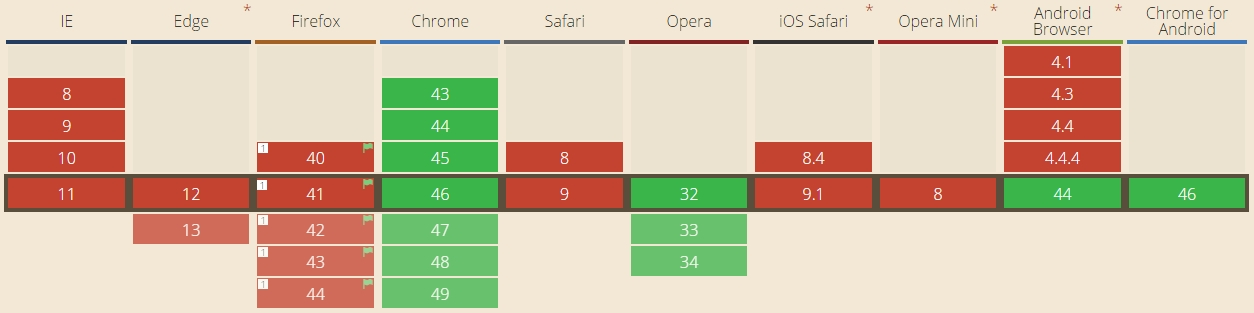
\includegraphics[width=\linewidth]{kapitel2/bilder/5-html-imports-browserunterstuetzung}
 \caption{Browserunterstützung der HTML Imports}
 \label{fig:bdhtmli}
\end{figure}


\section{Polyfills}\label{polyfills-mit-webcomponents.js}

In den Abschnitten \ref{custom-elements} bis \ref{html-imports} wurde gezeigt, wie die Web-Components-Technologien funktionieren und ob diese bereits in allen Browsern unterstützt werden. In diesem Abschnitt wird genauer darauf eingegangen was Polyfills sind. Ebenso wird auf deren Performance eingegangen und wie sie die Browserunterstützung der Web-Components-Technologien verbessern.


\subsection{Native Browserunterstützung von Web Components}\label{native-browserunterstuxfctzung-von-web-components}

In den einzelnen Unterkapiteln zu den Technologien wurde jeweils kurz gezeigt, ob diese von den Browsern unterstützt wird oder nicht. Es wurde deutlich, dass Chrome und Opera bisher die einzigen Vorreiter sind. Bis auf \ac{HTML} Templates, welche von allen modernen Browsern unterstützt werden, unterstützen sie als einzige alle Technologien. \cite{citeulike:13914379}

\begin{description}
  \item[Chrome] Hat alle Spezifikationen der Web-Component-Standards ab Version 43 komplett implementiert.
  \item[Firefox] Unterstützt nativ \ac{HTML} Templates. Custom Elements und Shadow \ac{DOM} sind zwar implementiert, müssen aber über das Flag \texttt{dom.webcomponents.enabled} manuell in den Entwicklereinstellungen aktiviert werden. \ac{HTML} Imports werden, wie in Kapitel \ref{html-imports} erwähnt, bis auf Weiteres nicht unterstützt.
  \item[Safari] \ac{HTML} Templates werden ab Version 8 unterstützt, Custom Elements und Shadow \ac{DOM} befinden sich in der Entwicklung (Stand Januar 2016), \ac{HTML} Imports werden jedoch nicht unterstützt.
  \item[Internet Explorer] Als einziger Browser unterstützt der Internet Explorer keine der Web-Components-Technologien. Die Unterstützung wird -- auf Grund der Einstellung der Entwicklung und des Wechsels zu Microsoft Edge -- auch nicht nachträglich implementiert werden.
  \item[Microsoft Edge] Templates werden ab Version 13 unterstützt, über die Entwicklung der restlichen Technologien kann allerdings abgestimmt werden \cite{citeulike:13914237}.
  \item[Mobile Browser] Alle Technologien werden bisher nur auf Android in den Browsern Chrome für Android, Opera und Android Browser unterstützt.
\end{description}

Die Browserunterstützung der Technologien der Web Components ist momentan also noch verhalten. Das bedeutet jedoch nicht, dass sie noch nicht verwendet werden können. Mittels JavaScript besteht die Möglichkeit, die Technologien den Browsern beizubringen, welche sie nicht unterstützen. Ein solches JavaScript wird ``Polyfill'' genannt.


\subsection{Polyfill webcomponents.js}\label{polyfill-webcomponents.js}

\begin{quote}
A polyfill, or polyfiller, is a piece of code (or plugin) that provides the technology that you, the developer, expect the browser to provide natively. \cite{citeulike:13914241}
\end{quote}

Mit Hilfe von Polyfills können die Technologie-Lücken der Browser also auf mehrere, unterschiedliche Arten (``Poly'') gefüllt (``fill'') werden \cite{citeulike:13914234}. Eine Sammlung an Polyfills Technologien der Web Components bildet das JavaScript webcomponents.js. Es wurde von Google im Rahmen von Polymer entwickelt und hat eine dermaßen weite Verbreitung erfahren, dass es auszugliedern wurde. Somit kann es auch unabhängig von der Benutzung von Polymer eingesetzt werden \cite{citeulike:13914239}.


\subsection{Browserunterstützung}\label{polyfills-browserunterstuetzung}

Mit dem Einsatz der webcomponents.js Polyfills werden die Web Components auch auf den Internet Explorer, Firefox sowie Safari portiert. Eine detaillierte Matrix der Browserunterstützung der Web Components mit Einsatz der Polyfills ist in Abbildung \ref{fig:bdwctmwcjs} \cite{citeulike:13914238} dargestellt.

\begin{figure}[htbp]
 \centering
 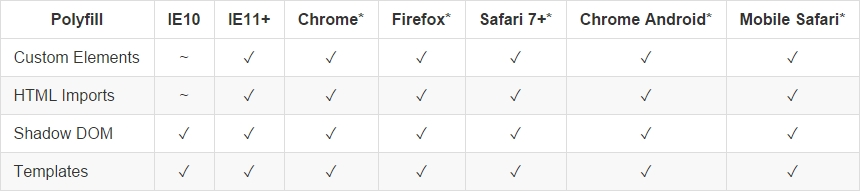
\includegraphics[width=\linewidth]{kapitel2/bilder/6-webcomponentsjs-browserunterstuetzung}
 \caption{Browserunterstützung der Web Components Technologien mit webcomponents.js}
 \label{fig:bdwctmwcjs}
\end{figure}

Jedoch werden die Technologien der Web Components auch mit Einsatzes der Polyfills nur von den aktuelleren Versionen des jeweiligen Browsers unterstützt. Darunter fallen jedoch weiterhin nicht ältere Browser, wie beispielsweise der Internet Explorer in Version 8 und 9. Des Weiteren werden einige Technologien auf Grund der Komplexität nicht komplett simuliert. Hier muss bei einigen Technologien auf folgende Punkte geachtet werden.

\begin{description}
  \item[Custom Elements] Die \ac{CSS}-Pseudoklasse \texttt{:unresolved} wird nicht unterstützt.
  \item[Shadow \ac{DOM}] Das Shadow \ac{DOM} kann auf Grund der Kapselung nicht komplett künstlich simuliert werden, dennoch versucht das webcomponents.js Polyfill einige der Features zu simulieren. So sprechen definierte \ac{CSS}-Regeln alle Elemente in einem künstlichen Shadow Root an -- als würde man den \texttt{\textgreater{}\textgreater{}\textgreater{}} Selektor benutzen -- auch die \texttt{::shadow} und \texttt{::content} Pseudoelemente verhalten sich so.
  \item[\ac{HTML} Templates] Templates, welche mit einem Polyfill erzeugt werden, sind nicht unsichtbar für den Browser, ihre enthaltenen Ressourcen werden also schon beim initialen Laden der Seite heruntergeladen.
  \item[\ac{HTML} Imports] Die zu importierenden \ac{HTML}-Dateien werden mit einem \ac{XHR}, und somit asynchron heruntergeladen, selbst wenn das \texttt{async}-Attribut (siehe Abschnitt \ref{asynchrones-laden-von-imports}) nicht gesetzt ist.
\end{description}


\subsection{Performance}\label{performance}

Das webcomponents.js-JavaScript \cite{citeulike:13914238} bringt mit seiner Größe von 116 KB einen großen Umfang mit, was sich negativ auf die Ladezeiten der Webseite auswirkt. Des Weiteren müssen die von den Browsern nicht unterstützten und ignorierten \ac{CSS}-Regeln -- wie \texttt{::shadow} oder \texttt{::slotted} -- mit Regular Expressions nachgebaut werden, was momentan 40 Stück sind. Das macht die Polyfills extrem komplex und träge. Die Funktionen zum Traversieren des \ac{DOM}s müssen angepasst werden, damit nur die richtigen Elemente angezeigt werden und eine Shadow Boundary simuliert wird. Diese werden mit 42 Wrappern umgesetzt, was wie die Regular Expressions zur Simulation der \ac{CSS}-Regeln sehr aufwändig ist. Allerdings können einige Funktionen wie \texttt{window.document} schlichtweg nicht überschrieben werden. Im Allgemeinen wird die \ac{DOM}-\ac{API} stark verlangsamt, wodurch die Performance -- speziell auf mobilen Geräten -- drastisch sinkt und mitunter nicht tolerierbar ist \cite{citeulike:13886251}.


\subsection{\texorpdfstring{Request-Minimierung mit ``Vulcanize''}{Request-Minimierung mit Vulcanize}}\label{request-minimierung-mit-vulcanize}

Webseiten können viele verschiedene, modular aufgebaute JavaScript-Dateien, Stylesheets, etc. beinhalten, welche die Anzahl an Requests erhöhen. Um die Anzahl an Requests zu verringern gibt es in der Webentwicklung bereits mehrere verschiedene Hilfsmittel. So werden die einzelnen Stylesheets oder auch JavaScript Dateien zu einer einzigen Datei konkateniert, sodass für das komplette Styling und JavaScript jeweils eine große Datei entsteht, welche nur einen Request an den Server benötigen. Zusätzlich kann sie anschließend noch minifiziert werden, um ihre Größe zu verringern und die Ladezeiten zu verkürzen. Selbiges Prinzip kann auch auf die \ac{HTML} Imports angewendet werden. Google stellt hierfür das Tool Vulcanize \cite{citeulike:13879681} bereit, welches serverseitig ermöglicht, einzelne kleine Web Components in einer einzigen, großen Web Component zusammenzufassen. Benannt nach der Vulkanisation, werden metaphorisch die einzelnen Elemente in ein beständigere Materialien umgewandelt. Vulcanize reduziert dabei eine \ac{HTML}-Datei und ihre zu importierenden \ac{HTML}-Dateien in eine einzige Datei. Somit werden die unterschiedlichen Requests in nur einem einzigen gebündelt und die Ladezeiten sowie die benötigte Bandbreite minimiert.


\section{Implementierung einer Komponente mit den nativen Web-Component-APIs}\label{implementierung-einer-komponente-mit-den-nativen-web-component-apis}

Anhand der vorhergehenden Abschnitte wird in diesem Abschnitt die Implementierung der Web Komponente \texttt{\textless{}custom-element\textgreater{}} mit den nativen \ac{HTML} APIs erläutert. Diese soll dabei das Markup in einem Shadow \ac{DOM} kapseln und den übergebenen Inhalt darstellen. Des Weiteren soll dessen Farbe über das Attribut \texttt{theme} optional konfiguriert werden können. Die gerenderte Komponente wird in Abbildung \ref{fig:gwkmnapis} dargestellt.

\begin{figure}[htbp]
 \centering
 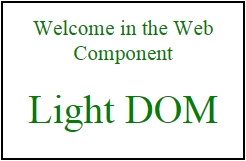
\includegraphics[width=5cm,keepaspectratio]{kapitel2/bilder/7-beispiel}
 \caption{Gerenderte Web Komponente mit nativen APIs}
 \label{fig:gwkmnapis}
\end{figure}


\subsection{Custom Element mit Eigenschaften und Funktionen definieren}\label{custom-element-mit-eigenschaften-und-funktionen-definieren}

Um ein neues Custom Element zu registrieren, wird zunächst ein \texttt{\ac{HTML}Element} Prototyp \texttt{CustomElementProto} mittels \texttt{Object.create(\ac{HTML}Element.prototype)} erstellt. Dieser wird anschließend um die Eigenschaft \texttt{theme} und dessen Standardwert \texttt{style1} erweitert, welches das deklarativ konfigurierbare
Attribut \texttt{theme} abbildet. Nun können die Lifecycle-Callback-Funktionen \texttt{createdCallback} und \texttt{attributeChangedCallback} der Komponente definiert werden (siehe Listing \ref{cemeufd}).

\lstinputlisting[language=JavaScript,label=cemeufd,caption=Custom Element mit Eigenschaften und Funktionen definieren]{kapitel2/listings/7-1.js}

Die \texttt{createdCallback}-Funktion soll zunächst prüfen ob das Attribut \texttt{theme} beim Verwenden des
\texttt{\textless{}custom-element\textgreater{}}-Tags verwendet und ein entsprechender Wert gesetzt wurde und übergibt dieses der Hilfsfunktion \texttt{setTheme}. Wird das Attribut nicht gesetzt, wird der Standardwert \texttt{style1} übergeben. Falls das \texttt{style}-Attribut von Außen geändert wird, soll die \texttt{attributeChangedCallback} Funktion gewährleisten, dass die Änderung auch von der Komponente übernommen wird, indem sie das Attribut der Hilfsfunktion \texttt{setTheme} übergibt. Um das Setzen und Ändern des \texttt{theme}-Attributs zu implementieren wird zuletzt die Hilfsfunktion \texttt{setTheme} für den Prototyp definiert (siehe Listing \ref{hsetthemed}).

\lstinputlisting[language=JavaScript,label=hsetthemed,caption=HilfsFunktion \texttt{setTheme} definieren]{kapitel2/listings/7-2.js}

Diese setzt den übergebenen Parameter, das \texttt{theme}-Attribut, als Klasse auf den umschließenden Wrapper \texttt{.outer}, welche dabei den zu verwendenden Style der Komponente bestimmt. Da der Prototyp nun alle erforderlichen Eigenschaften besitzt, kann er mit \texttt{document.registerElement(\dq custom-element\dq,\ \{\ prototype:\ CustomElementProto\ \});} als \ac{HTML}-Tag \texttt{custom-element} in dem importierenden Dokument verfügbar gemacht werden.


\subsection{Template erstellen und Styles definieren}\label{template-erstellen-und-styles-definieren}

Bisher ist das Custom Element zwar funktional, bietet aber noch kein gekapseltes Markup. Hierfür wird ein Template mit der ID \texttt{myElementTemplate} angelegt (siehe Listing \ref{teusd}), welches die für die Komponente notwendige \ac{HTML} Struktur beinhaltet.

\lstinputlisting[language=HTML,label=teusd,caption=Template erstellen und Styles definieren]{kapitel2/listings/7-3.html}

Das Template enthält dabei einen Insertion Point \texttt{\textless{}content\textgreater{}}, in welchem die Kind-Elemente der Komponente in das interne Markup projiziert werden. Zusätzlich werden 2 Hilfs-Wrapper und Text definiert, damit die Elemente schneller mittels JavaScript selektierbar sind und das gewünschte Aussehen erreicht wird. Um nun die verschiedenen Styles, welches mittels dem \texttt{theme}-Attribut ausgewählt werden kann, zur Verfügung zu stellen, werden diese in einem \texttt{\textless{}style\textgreater{}}-Tag in dem Template definiert. In diesem Beispiel werden 2 Optionen, \texttt{style1} und \texttt{style2} zur Verfügung gestellt, sowie weitere Styles für die gesamte Komponente definiert (siehe Listing \ref{stylesdefinieren}).

\lstinputlisting[language=HTML,label=stylesdefinieren,caption=Styles definieren]{kapitel2/listings/7-4.html}

Das Template wird nun zwar schon heruntergeladen, jedoch noch nicht in den \ac{DOM} eingefügt. Hierzu muss es dem Shadow Root hinzugefügt werden, was in dem nachfolgenden Abschnitt \ref{template-bereitstellen-und-shadow-dom-zur-kapselung-benutzen} dargestellt wird.


\subsection{Template bereitstellen und Shadow DOM zur Kapselung benutzen}\label{template-bereitstellen-und-shadow-dom-zur-kapselung-benutzen}

Bevor das erstellte Template eingebunden werden kann, muss zunächst ein Shadow Root mittels \texttt{var\ shadow\ =\ this.createShadowRoot();} erzeugt werden. Hierfür wird die bereits definierte Lifecycle-Callback-Funktion \texttt{createdCallback} erweitert. Somit kann der Shadow \ac{DOM} sofort initialisiert werden, wenn das Element erzeugt wurde. Nun kann der Inhalt des Templates mit der ID \texttt{myElementTemplate} mittels \texttt{var\ template\ =\ importDoc.querySelector('\#myElementTemplate').content;} importiert und mit der Anweisung \texttt{shadow.appendChild(template.cloneNode(true));} dem Shadow Root hinzugefügt werden. Die Variable \texttt{importDoc} stellt dabei die Referenz auf die importierte Komponente, also das \texttt{\textless{}custom-element\textgreater{}}-Element, dar und kann mittels der Funktion \texttt{var\ importDoc\ =\ document.currentScript.ownerDocument;} ermittelt werden. Wird dies nicht getan, so würde der \texttt{querySelector} auf das Eltern-Dokument der eingebetteten Komponente zugreifen und das Template nicht finden. Nun ist der Inhalt des Templates als Shadow \ac{DOM} innerhalb des Elements gekapselt und nach Außen nicht sichtbar.

\subsection{Element importieren und verwenden}\label{element-importieren-und-verwenden}

Das Element ist somit vollständig und kann in einer beliebigen Webseite oder Applikation eingesetzt werden. Hierzu muss das Element mittels \texttt{\textless{}link\ rel=\dq import\dq\ href=\dq elements/custom-element.html\dq\textgreater{}} zunächst importiert werden. Es kann anschließend mit entsprechenden Attributen und Inhalt auf der Seite eingebettet werden, wie beispielsweise der Konfiguration \texttt{\textless{}custom-element\ theme=\dq style1\dq\textgreater{}Light DOM\textless{}/custom-element\textgreater{}}. Das vollständige Beispiel der Komponente, sowie dessen Einbindung in ein \ac{HTML}-Dokument sind im Anhang zu finden. \todo{referenz}




% Abkuerzungsverzeichnis
\section{Abkürzungsverzeichnis}
\begin{acronym}

 \acro{bzw.}{beziehungsweise}
 \acro{HTML}{Hypertext Markup Language}
 \acro{W3C}{World Wide Web Consortium}
 \acro{DOM}{Document Object Model}
 \acro{CSS}{Cascading Style Sheets}
 \acro{API}{Application Programming Interface}
 \acro{FOUC}{Flash Of Unstyled Content}
 \acro{LIFO}{Last In First Out}

\end{acronym}
\end{document}


\listoffigures
\lstlistoflistings

% REMOVE THIS!
\listoftodos[TODOs]
% REMOVE THIS!

\bibliographystyle{apalike-mystyle}
\bibliography{library}
\end{document}

